% Appendix
\chapter{Appendix}


\seb{change appendix name or way it is displayed. I want to have just 1 appendix}

\begin{figure}[H]
  \centering
  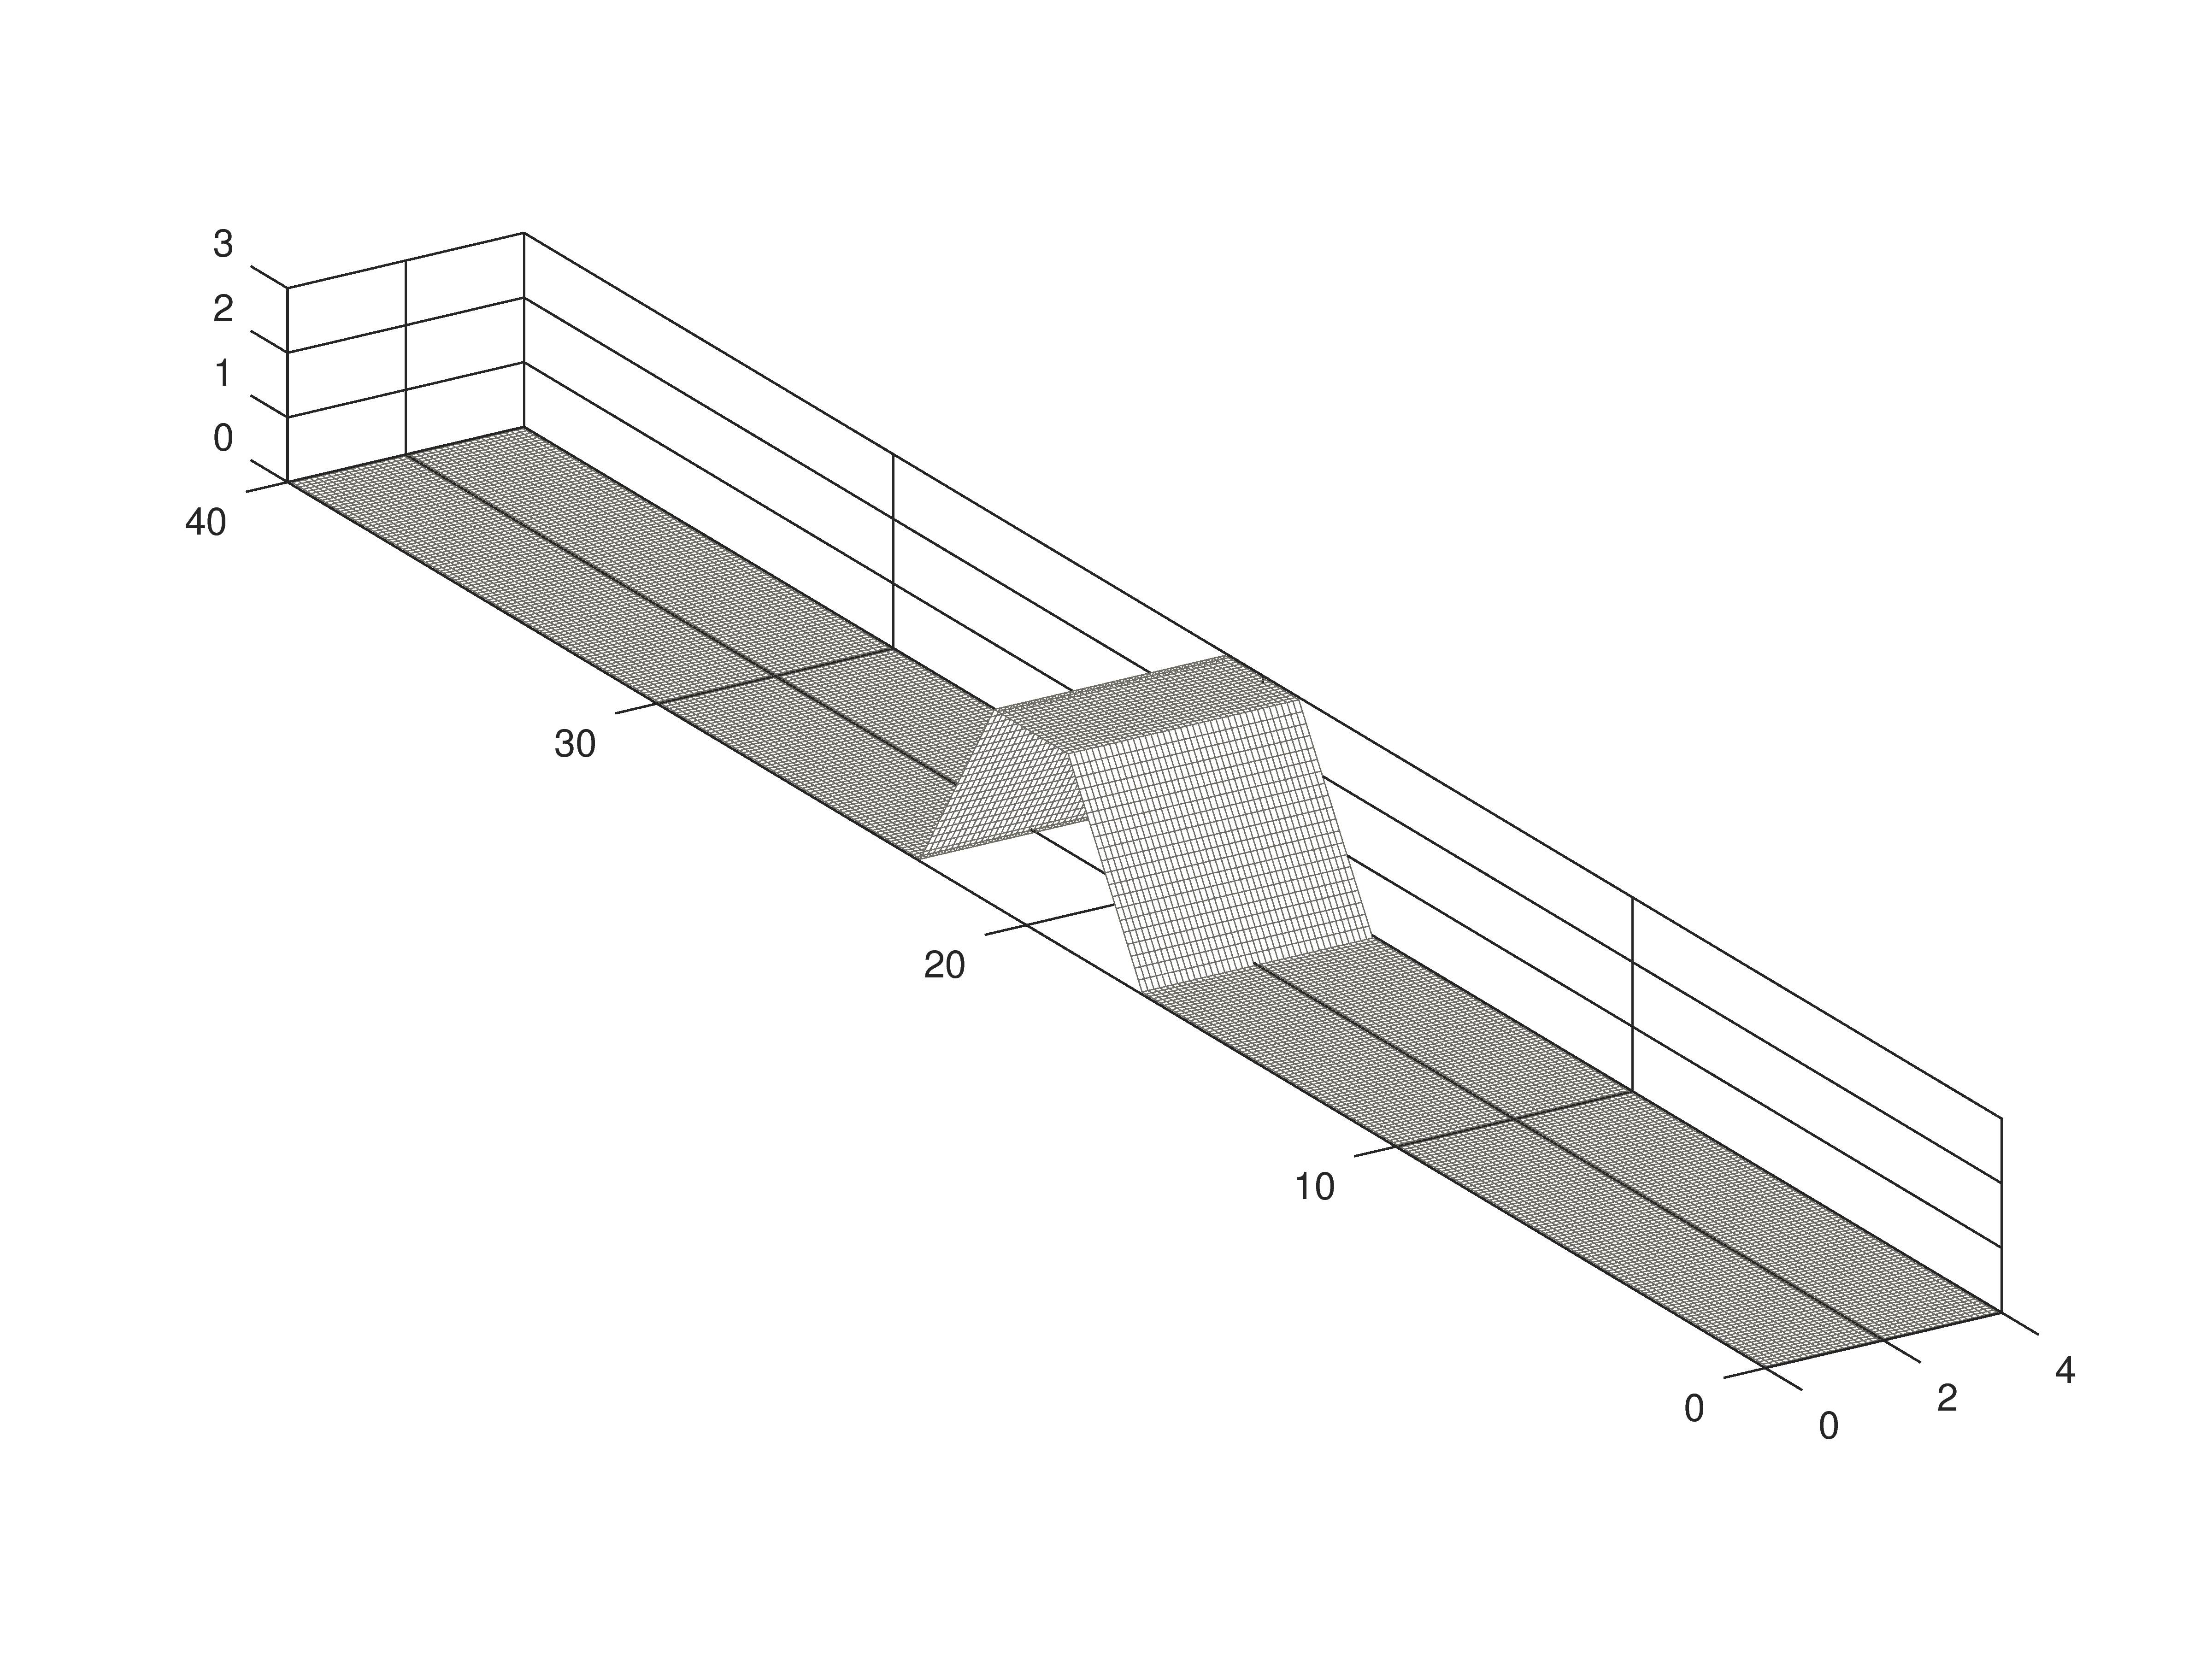
\includegraphics[width=0.8\textwidth]{Figures/channel.png}
  \caption{Topography of the channel used for \emph{case study 1}. The channel presents no walls because "wall boundary conditions" were chosen in \textit{FullSWOF\_2D} for the two lateral boundaries.}
  \label{fig:channel}
\end{figure}
\seb{does it make sense to put this figure?}


\begin{figure}[H]
  \centering
  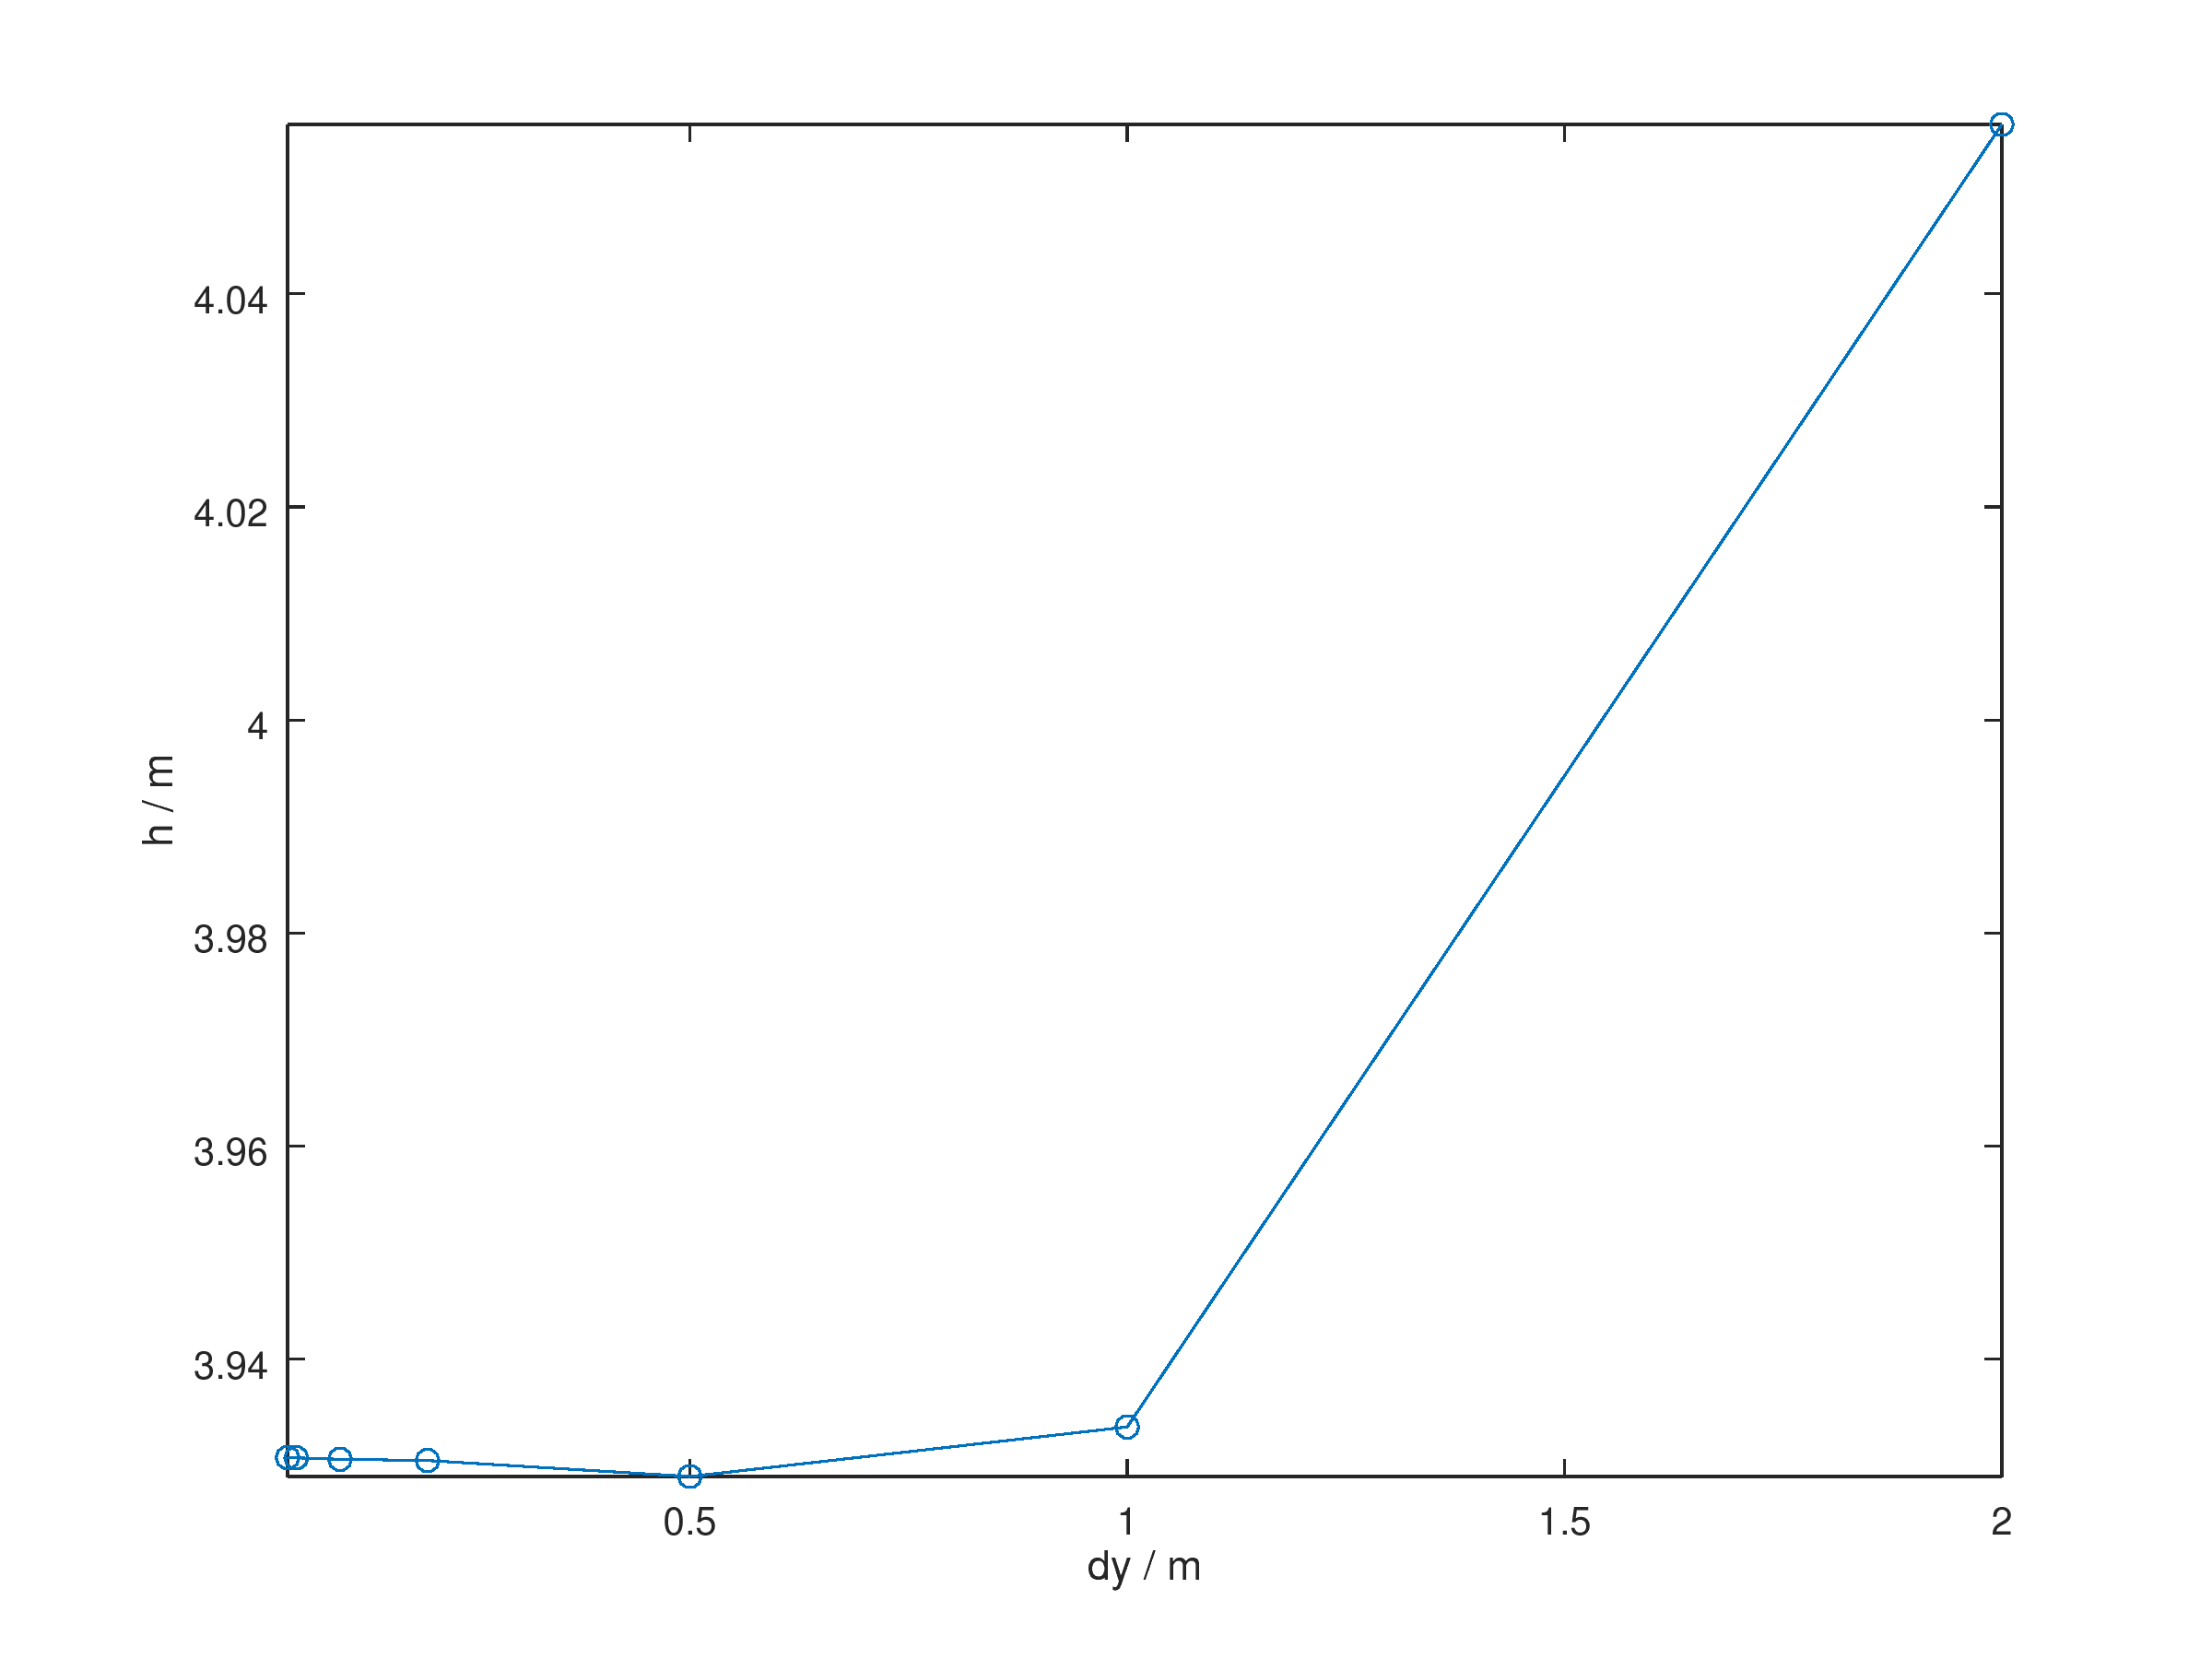
\includegraphics[width=0.7\textwidth]{Figures/convergence_center.png}
  \caption{Measured free surface height at the weir midpoint as a function of the grid resolution used.}
  \label{fig:convergence_center}
\end{figure}


\begin{table}[htpb]
  \centering
  \caption{Dataset used for computing the model error.}
  \label{tab:dataset_error}
  \begin{tabular}{lcr}
    \toprule
    header1 & header2 & header3 \\
    \midrule
    item11 & item12 & item13 \\
    item21 & item22 & item23 \\
    \bottomrule
  \end{tabular}
\end{table}


\begin{table}[H]
  \centering
  \caption{Emulator training dataset}
  \label{tab:training_dataset}
  \begin{tabular}{lccc}
    \toprule
     & \textbf{1} & \textbf{2} & \textbf{3}\\
    \midrule
    $\bm{I}$ \textbf{[\si{\milli\meter\per\hour}]} & val & val & val \\
    $\bm{\theta_i}$ \textbf{[--]} & val & val & val \\
    \bottomrule
  \end{tabular}
\end{table}


\begin{table}[H]
  \centering
  \caption{Emulator test dataset}
  \label{tab:test_dataset}
  \begin{tabular}{lccc}
    \toprule
     & \textbf{1} & \textbf{2} & \textbf{3}\\
    \midrule
    $\bm{I}$ \textbf{[\si{\milli\meter\per\hour}]} & val & val & val \\
    $\bm{\theta_i}$ \textbf{[--]} & val & val & val \\
    \bottomrule
  \end{tabular}
\end{table}


\begin{table}[H]
  \centering
  \caption{Emulator validation dataset}
  \label{tab:validation_dataset}
  \begin{tabular}{lccc}
    \toprule
     & \textbf{1} & \textbf{2} & \textbf{3}\\
    \midrule
    $\bm{I}$ \textbf{[\si{\milli\meter\per\hour}]} & val & val & val \\
    $\bm{\theta_i}$ \textbf{[--]} & val & val & val \\
    \bottomrule
  \end{tabular}
\end{table}


\begin{table}[H]
  \centering
  \caption{Emulator performance on every validation point}
  \label{tab:validation_performance}
  \begin{tabular}{lccc}
    \toprule
     & \textbf{1} & \textbf{2} & \textbf{3}\\
    \midrule
    \textbf{simulated} $\bm{t_!}$ & val & val & val \\
    \textbf{emulated} $\bm{t_!}$ & val & val & val \\
    \bottomrule
  \end{tabular}
\end{table}
